\subsection{Datenextraktion aus dem Web}
Das Web stellt eine der wichtigsten Quellen der unstrukturierten und semi-strukturierten Daten dar. Es wurden zahlreiche Methoden der Datenextraktion aus dem Web entwickelt, die in unterschiedlichen Anwendungsbereichen eingesetzt werden. Ferrara et al unterscheiden dabei zwei Kategorien der Algorithmen zur Datenextraktion, n�mlich Tree Matching Algorithmen und Algorithmen des maschinellen Lernens \cite[S.302]{ferrara2014}. Da das maschinelle Lernen wird explizit im Abschnitt \ref{subsec: Maschinelles-Lernen} angesprochen, wird im Weiteren ein Beispiel eines Tree Matching Algorithmus betrachtet.\\
Aufgrund der Struktur der Webressourcen ist die Erfassung der Daten aus dem Web nicht einfach. Ferrara et al nennen folgende Herausforderungen, die bei der Datenerfassung aus Webressourcen vorkommen \cite[S.302]{ferrara2014}:
\begin{itemize}
\item \textit{Automatisierungsgrad}: Die Erfassung der Webdaten soll oft von einem menschlichen Experten �berwacht werden, um die Genauigkeit der Daten zu gew�hrleisten.
\item \textit{Skalierbarkeit}: Bei den umfangreichen Webressourcen soll innerhalb k�rzer Zeit schnell eine gro�e Datenmenge bearbeitet werden.
\item \textit{Datenschutz}: Wenn es um die Erfassung der personenbezogenen Daten geht (bei sozialen Netzwerken wie Facebook), soll die Privatsph�re des Individuums nicht beeintr�chtigt werden.
\item \textit{�nderung der Ressourcenstruktur}: Die Struktur der Webressourcen �ndert sich oft. Die Datenerfassungsmethoden f�r das Web sollen eine gewisse Flexibilit�t besitzen, um weiterhin korrekt zu funktionieren.
\item \textit{Trainingsdaten}: Das maschinelle Lernen braucht eine Trainingsmenge der Webseiten, die manuell mit Labels annotiert werden. Dies ist eine schwierige und fehleranf�llige Aufgabe.
\end{itemize}
Ein Verfahren, das am meisten zur Datenerfassung aus dem Web bekannt ist, nutzt die semi-strukturierten Dokumente, die in \acf{HTML} beschrieben werden. Eine HTML-Seite wird in \acf{DOM}\footnote{https://www.w3.org/DOM} definiert. Die Idee vom DOM besteht darin, dass die HTML-Webseite ein Baum darstellt, der mittels HTML-Tags (z.B. Button-Tag) ausgezeichnet wird. Tags k�nnen weitere Tags beinhalten und bilden somit eine hierarchische Struktur. Diese hierarchische Baumstruktur erm�glicht effiziente Datensuche in einer HTML-Seite \cite[S.303]{ferrara2014}.\\
Da HTML ein Dialekt von \acf{XML} ist, kann \acf{XPath}\footnote{https://www.w3.org/TR/xpath} f�r die Navigation in DOM eingesetzt werden. In einem XPath-Ausdruck k�nnen beliebige Elemente einer HTML-Webseite ausgew�hlt werden. In Abbildung \ref{xpath} werden zwei Beispiele dargestellt. Im ersten Fall (A) wird genau ein Element (die erste Zelle in der ersten Reihe) ausgew�hlt. Im Beispiel (B) werden mehrere Elemente (alle Zellen der zweiten Reihe) angesprochen \cite[S.303]{ferrara2014}.
\begin{figure}[H] 
	\centering
	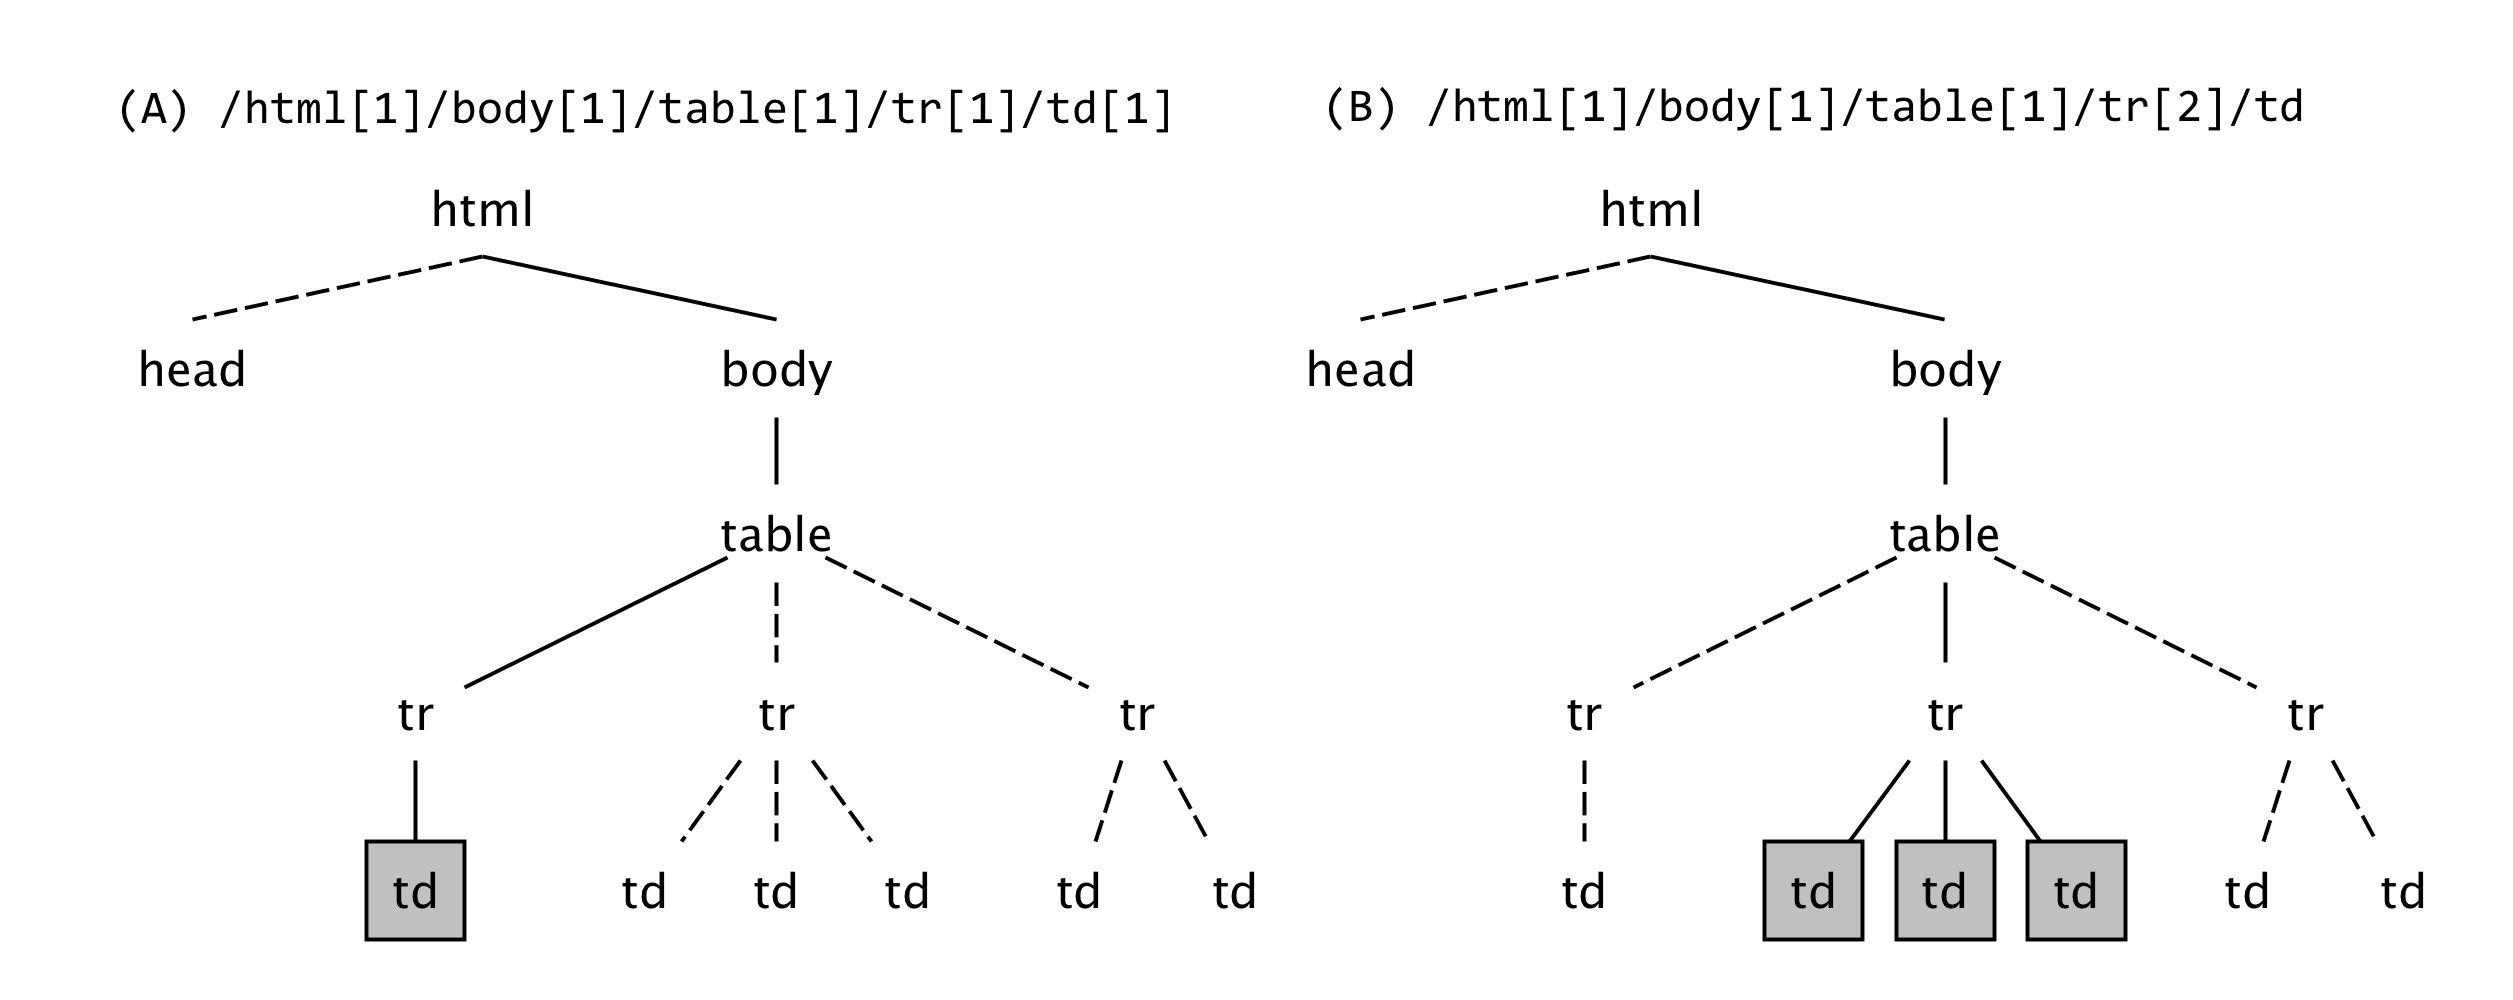
\includegraphics[width=1.0\textwidth]{images/xpath.png}
	\caption{XPath im Dokumentenbaum, \cite[S.304]{ferrara2014}}
	\label{xpath}
\end{figure} 
Der Hauptnachteil von XPath besteht darin, dass XPath-Ausdr�cke strikt an der DOM-Struktur gebunden sind. Wenn eine �nderung im DOM stattfindet, funktioniert der von der �nderung betroffene Ausdruck nicht mehr. Aus diesem Grund m�ssen die XPath-Ausdr�cke nach jeder Ver�nderung der HTML-Webseite manuell angepasst werden. In Bezug auf dieses Problem wurde im letzten Release von XPath\footnote{https://www.w3.org/TR/xpath20} relative XPath-Ausdr�cke eingef�hrt \cite[S.304]{ferrara2014}.\\
Eine Beispiel des Verfahrens zur Datenextraktion ist ein Web Wrapper. Unter dem Web Wrapper wird ein Verfahren verstanden, das eine oder mehrere Algorithmen zur Datensuche beinhaltet. Dabei werden die Daten in unstrukturierten oder semi-strukturieren Dokumenten erfasst und in eine strukturierte Form transformiert. Ein Wrapper-Lebenszyklus umfasst folgende Schritte \cite[S.305]{ferrara2014}:
\begin{itemize}
\item[1.]\textit{Generierung}: Definition des Wrappers.
\item[2.]\textit{Ausf�hrung}: Datenerfassung mithilfe des Wrappers.
\item[3.]\textit{Wartung}: Anpassung des Wrappers bei der �nderung der DOM-Struktur.
\end{itemize}
Nach Ferrara et al kann ein Web Wrapper unter Verwendung von regul�ren Ausdr�cken, logikbasiertem Ansatz, Baumansatz oder maschinellem Lernen generiert werden \cite[S.306]{ferrara2014}. Im Weiteren wird der Ansatz von regul�ren Ausdr�cken im Rahmen des zweiten Schritts (Ausf�hrung) verdeutlicht.\\
Regul�re Ausdr�cke erm�glichen die Erkennung von Patterns in der unstrukturierten bzw. semi-strukturierten Dokumenten mithilfe der Regeln, die z.B. in Form von Wortgrenzen oder HTML-Tags definiert werden. Der Vorteil der regul�ren Ausdr�cken besteht darin, dass der Benutzer die Elemente auf einfache Weise in einem grafischen Interface ausw�hlen kann. Die dazugeh�rigen Regeln werden dann automatisch generiert. Eine m�gliche Umsetzung des Wrappers wird in \cite{sahuguet1999} mit W4F vorgestellt. Das Tool verf�gt �ber eine Hilfsmethode, die den Benutzer bei der Auswahl der Elementen unterst�tzt. Auf Basis der ausgew�hlten Elementen werden die Regeln erstellt. Allerdings sind die Regeln in Bezug auf DOM-�nderungen nicht flexibel. Dies f�hrt dazu, dass die Regeln stets von einem menschlichen Experten angepasst werden sollen \cite[S.306]{ferrara2014}.\\
\textbf{Weiter mit Wartung ... }